%--------------------------------------------------------------------------------------------------
\begin{frame}
    \frametitle{Evaluating Interpretability}
    \framesubtitle{Three paradigms}
    \small
    \pause
    \begin{itemize}
        \item\textbf{Interpretable Image Recognition\cite{chattopadhay2018grad}}\\
             Average Drop (AD), Average Increase (AI), Average Gain (AG).\pause
        \item\textbf{Causality Analysis\cite{petsiuk2018rise}}\\
             Insertion \& Deletion.
        \item\textbf{Weakly Supervised Localization Approach}\\\pause
            Official Metric (OM), Localization Error (LE), Pixel-wise $F_1$ score (F1)
            Box Accuracy (BA), Standard Pointing Game (SP), Energy Pointing Game (EP).
    \end{itemize}
\end{frame}
%--------------------------------------------------------------------------------------------------
%\begin{frame}[t]
%    \frametitle{Evaluating Interpretability}
%    \framesubtitle{Interpretable Image Recognition}
%    \small
%    An explanation should demonstrate similar predictive properties to its query:\\
%    \begin{columns}
%        \column[T]{0.4\textwidth}
%            \begin{center}
%                {\scriptsize Input image. ($I$)}\\
%                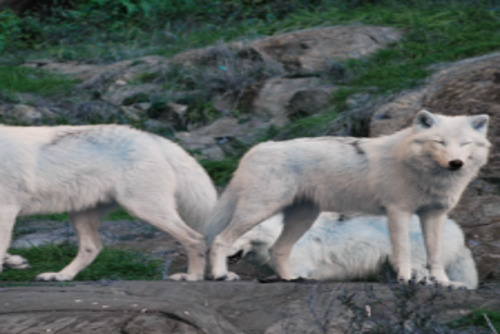
\includegraphics[width=.5\textwidth]{fig/rel/interp/img/ILSVRC2012_val_00000027.JPEG}\\
%                {\scriptsize $P^c_i = 0.8756$}\\
%            \end{center}
%        %\column{0.3\textwidth}
%            \begin{center}
%                {\scriptsize Explanation Map. ($E^c$)}\\
%                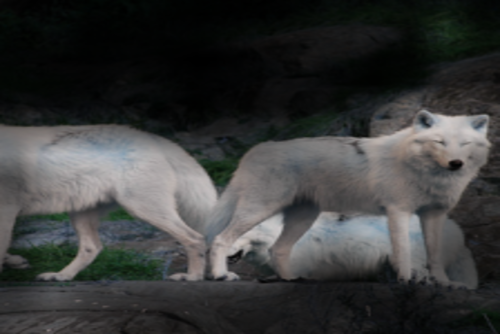
\includegraphics[width=.5\textwidth]{fig/rel/interp/img/masked_resized.png}\\
%                {\scriptsize $O^c_i = 0.7442$}
%            \end{center}
%        \pause
%        \column[T]{.6\textwidth}            
%            \vspace{10pt}
%                \begin{equation}
%                    \mbox{AD(\%)} \defn \frac{1}{N}\sum_{i=1}^N\frac{[y_i^c-o_i^c]_+}{y_i^c} \cdot 100    
%                \end{equation}
%                \pause
%                \begin{equation}
%                    \mbox{AI(\%)} \defn \frac{1}{N} \sum_i^N \mathds{1}_{y^c_i < o^c_i} \cdot 100
%                \end{equation}
%                \pause
%                \begin{equation}
%                    \mbox{AG(\%)} \defn \frac{1}{N}\sum_{i=1}^N\frac{[o_i^c-y_i^c]_+}{1-y_i^c} \cdot 100
%                \end{equation}
%            
%    \end{columns}
%\end{frame}
%--------------------------------------------------------------------------------------------------
%\begin{frame}[t]
%    \frametitle{Interpretability}
%    \framesubtitle{Causality Analysis}
%    \small
%    Saliency guided perturbations revelal the importance of salient regions.\\
%    \begin{columns}
%        \column[T]{0.4\textwidth}
%            \begin{center}
%                {\scriptsize Input image. ($I$)}\\
%                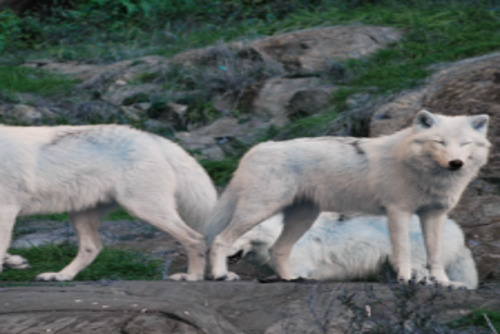
\includegraphics[width=.5\textwidth]{fig/rel/interp/img/ILSVRC2012_val_00000027.JPEG}\\
%            \end{center}
%        %\column{0.3\textwidth}
%            \begin{center}
%                {\scriptsize Saliency Map. ($E^c$)}\\
%                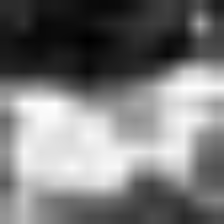
\includegraphics[width=.5\textwidth]{fig/rel/interp/img/saliency.png}\\
%            \end{center}
%        \pause
%        \column[T]{.6\textwidth}
%                \begin{itemize}
%                    \item \textbf{Insertion}: Blur the image, then reconstruct the original guided by saliency.\pause
%                    \item \textbf{Deletion}: Replace with zeros the image guided by Saliency
%                \end{itemize}
%    \end{columns}
%\end{frame}
%--------------------------------------------------------------------------------------------------